\documentclass{jsarticle}

\usepackage[dvipdfmx]{graphicx}
\usepackage{tabularx}
\usepackage{booktabs}
\usepackage[dvipdfmx]{xcolor}
\usepackage{listings} 
\usepackage{float} 

\title{Webプログラミング レポート課題}
\author{24G1091 田代 壮}
\date{}


\begin{document}
\maketitle
\pagenumbering{gobble}



\section{利用者向けの説明}

 ここでは,掲示板の利用方法について説明する.まず,掲示板には図1のように「名前」と「メッセージ」と書かれた隣にそれぞれ入力するスペースが表示されている.
掲示板に何か書き込む場合には適当な「名前」と「メッセージ」を入力
し,隣に「送信」と青い背景に囲まれたボタンが表示されているのでそこをクリックすることで掲示板に書き込むことができる.

\begin{figure}[H]
    \centering
    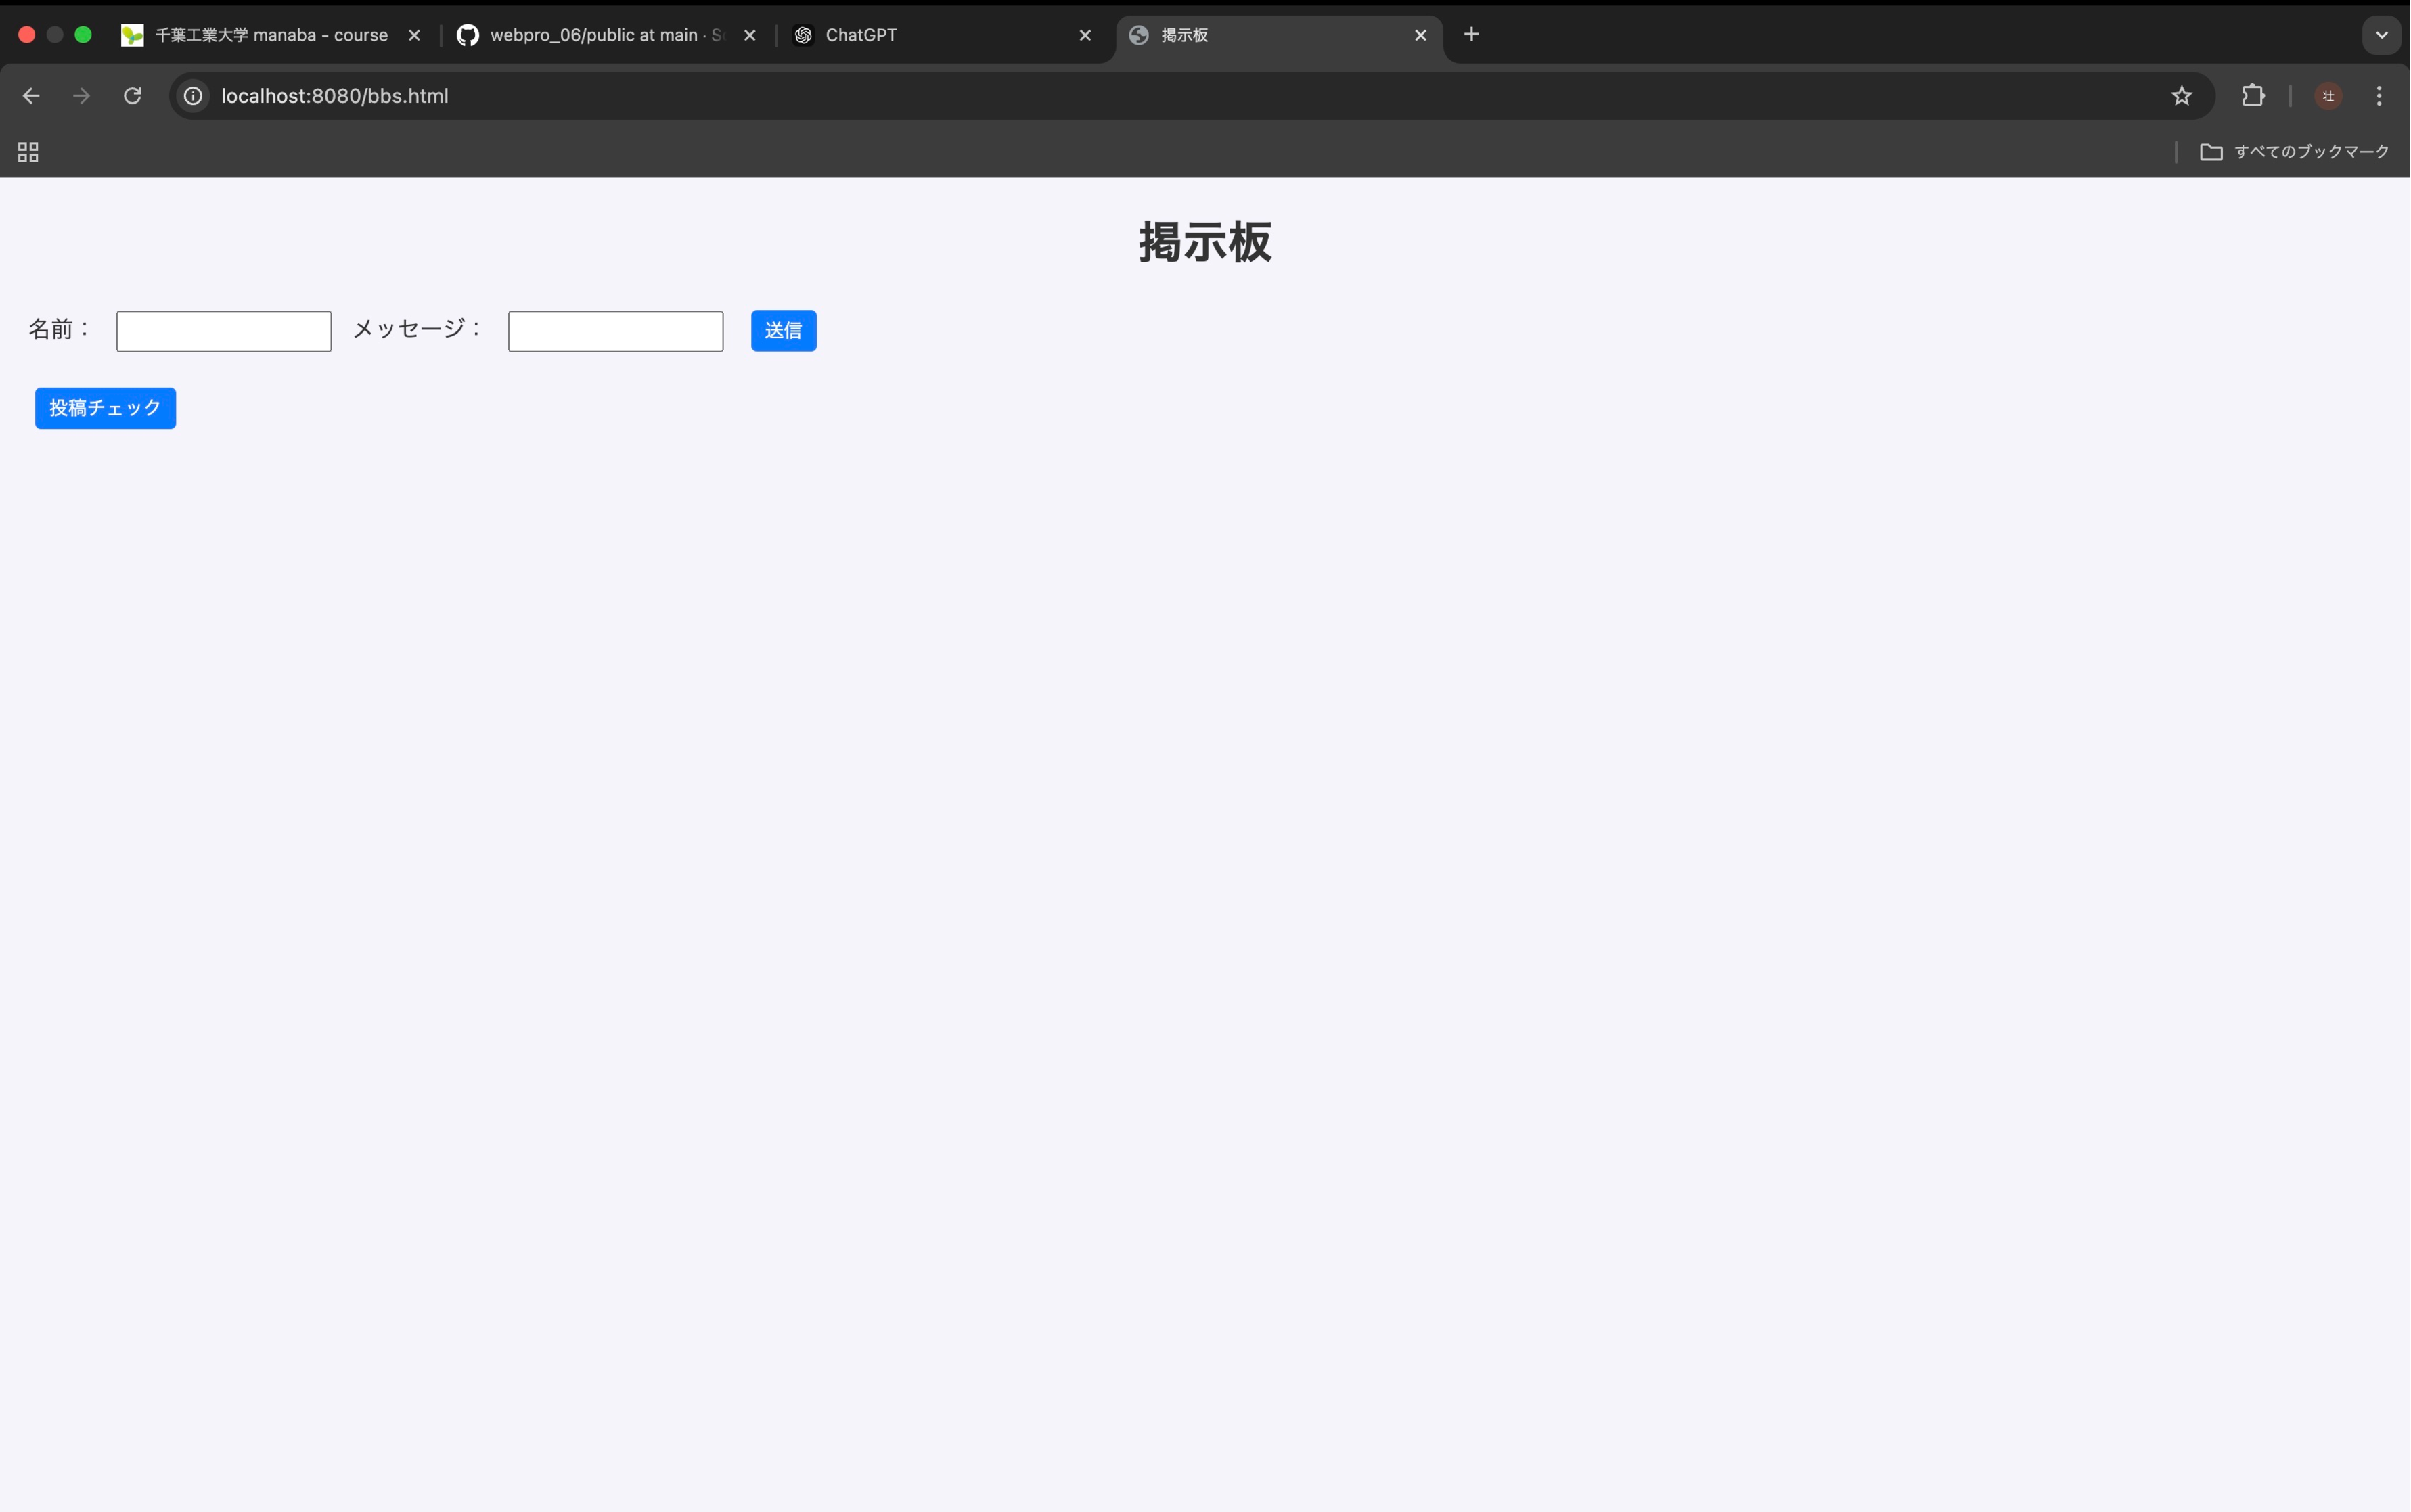
\includegraphics[width=10cm]{fig/keiji.pdf}
    \caption{掲示板の初期表示}
    \label{photoreflector_characteristic}
\end{figure}

書き込んだ投稿を確認する場合には,「名前」などの下に青い背景で囲まれている「投稿チェック」
というボタンが表示されているので,それをクリックすると投稿を確認することができる.

\begin{figure}[H]
    \centering
    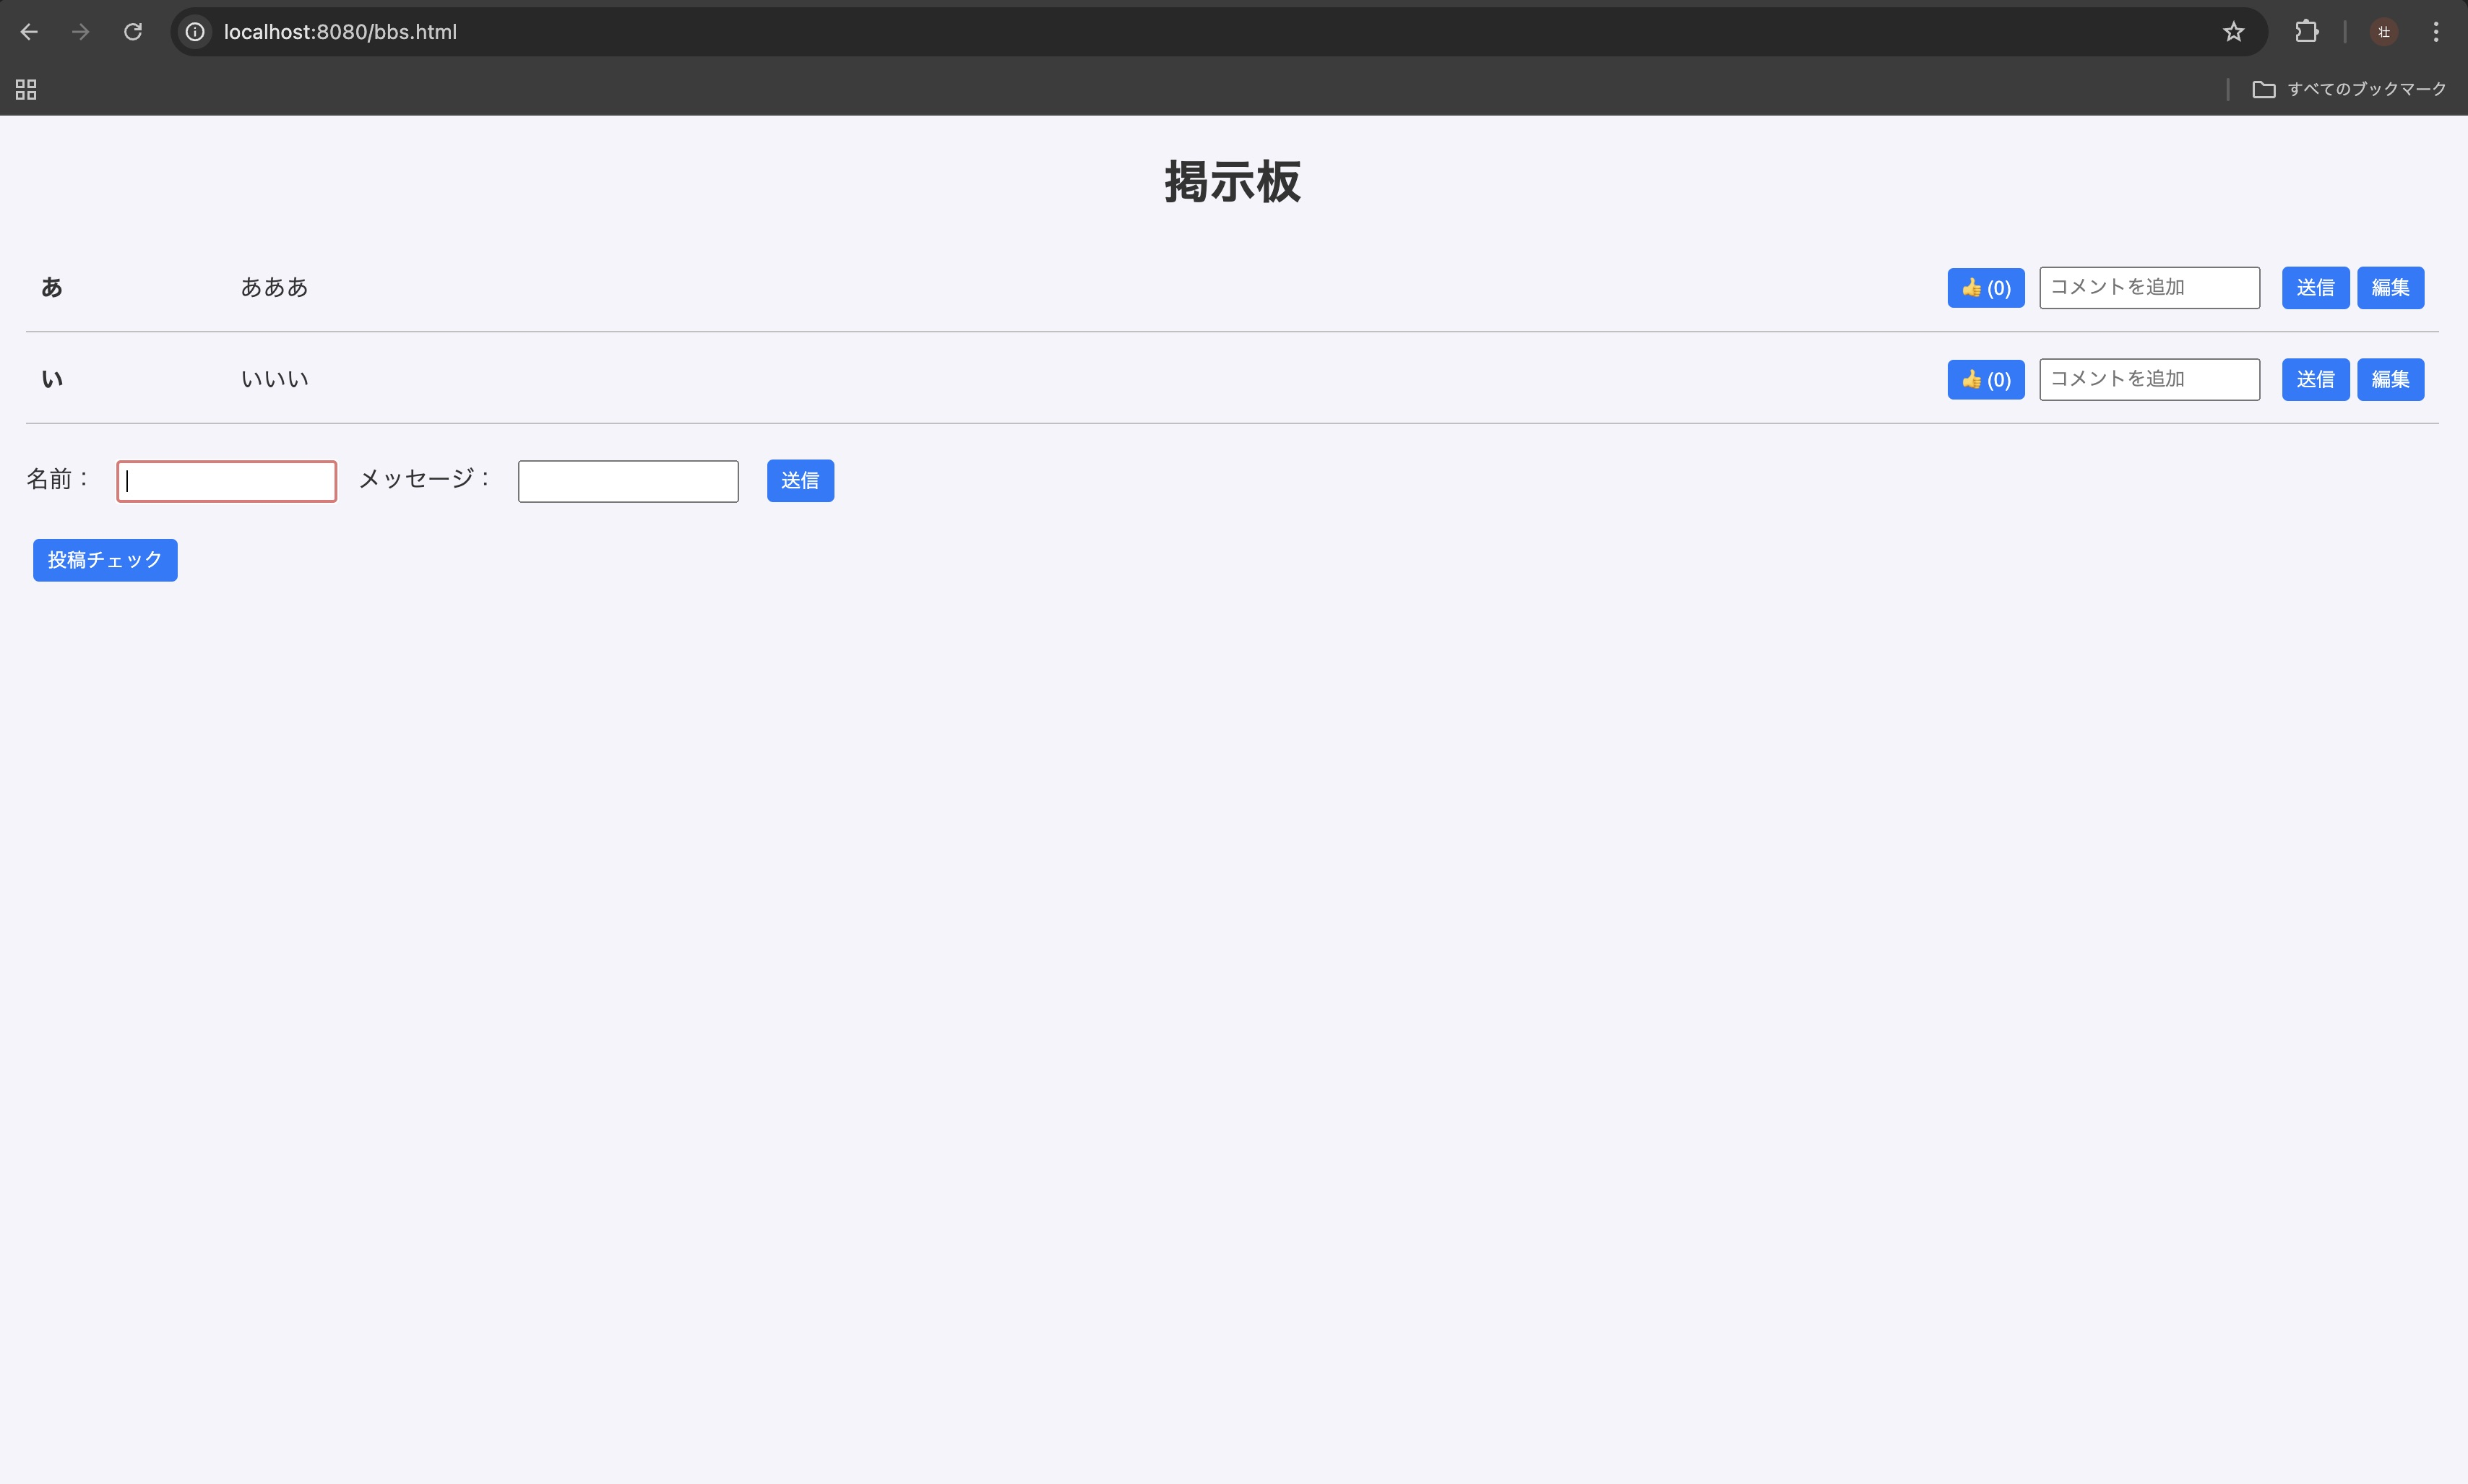
\includegraphics[width=10cm]{fig/check.jpeg}
    \caption{投稿チェック}
    \label{photoreflector_characteristic}
\end{figure}

 次に,掲示板に投稿された文章に対しての機能についての説明をする.投稿された文章に対しての機能は主に3つある.
投稿された文章には右端に青い背景で囲まれた「👍(0)」と「コメントを追加」という何か書くスペースと「送信」,そして「編集」というボタンが表示される.

\subsection{いいね機能}
各投稿には「いいね」ボタン(👍)があり,これを押すことでその投稿に「いいね」を追加することができる.「いいね」ボタンを押すことで「👍」の横にカウントされている数字が一つ増える.
また,「いいね」はカウント100まで送ることができる.

\subsection{コメント機能}
各投稿に対してコメントを入力するスペースがあり,他の投稿に対してコメントを送ることができる.コメントを入力して送信すると投稿に対してのコメントが追加される.
一つの投稿に対して複数のコメントを送信することができ,上から順番に表示される.


\subsection{投稿編集機能}
投稿編集機能とは投稿したメッセージを後から編集することができる機能である.自分の投稿した文章の右端にある編集ボタンを押すことで,投稿を編集することができる.
変更後の文章を入力して保存ボタンを押すことで変更が更新される.

\begin{figure}[H]
    \centering
    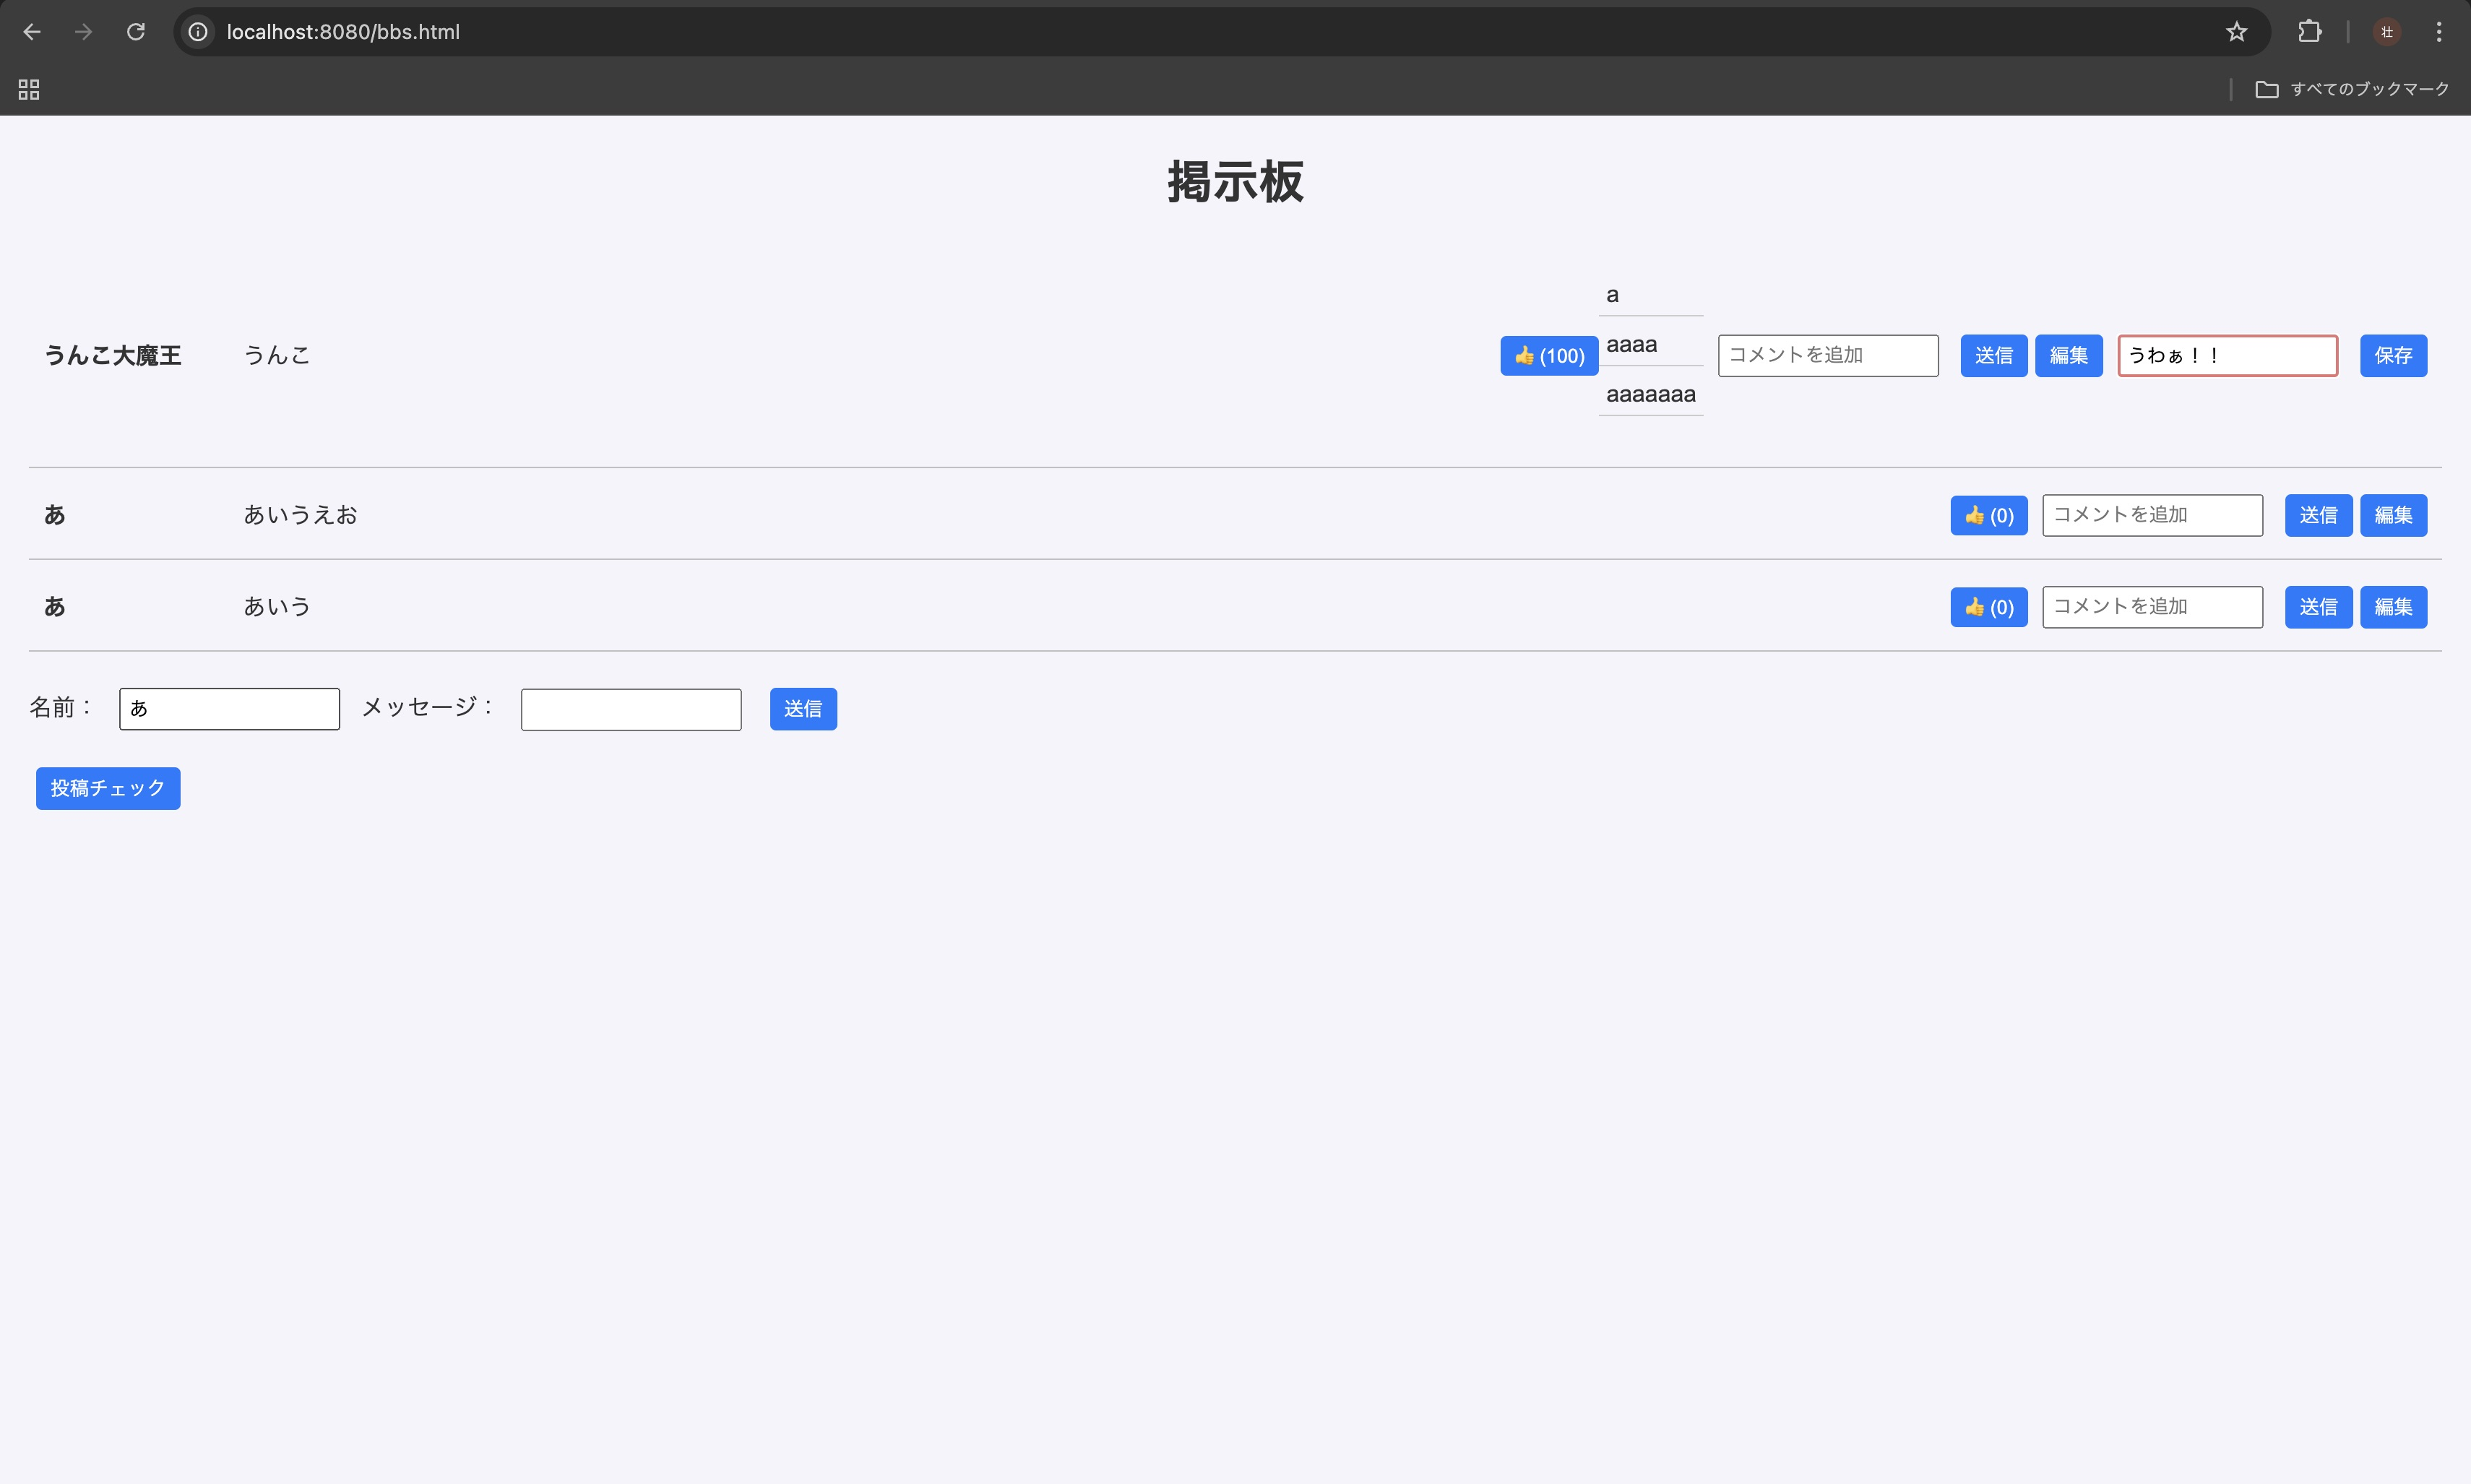
\includegraphics[width=10cm]{fig/kinou.jpeg}
    \caption{機能}
    \label{photoreflector_characteristic}
\end{figure}

\section{管理者向けの説明}

 まず,サーバを立ち上げるための準備としてnode.jsをインストールしておく.「node -v」,「npm -v」と順にターミナルで実行することでインストールされているかを確認することができる.
サーバを立ち上げる時には,「node app8.js」を実行することでサーバを立ち上げることができる.\par
サーバが起動すると,「Server is running at http://localhost:8080」と表示される.その後,ブラウザで「http://localhost:8080」を開くと,掲示板の動作を確認することができる.\par

\subsection{掲示板の動作}
掲示板にアクセスすることで,その度に新しい投稿が一覧で表示される.管理者はその投稿やコメントを閲覧することが出来る.

\subsection{いいね機能}
特定の投稿に「いいね」を追加するエンドポイント(POST /bbs/:id/like)にリクエストが来ると,指定された投稿の「いいね」数を一つ増やす.
流れとしては,投稿IDを受け取りそのIDに対応する投稿を検索し,見つかった投稿の「いいね」数を増やし,更新された「いいね」数をレスポンスとして返す.

\subsection{コメント機能}
(POST /bbs/:id/comment)は指定された投稿に対してのコメントを追加するエンドポイントである.投稿IDを受け取り,その投稿にコメントを追加する.
コメントリストを更新後にレスポンスとして返す.

\subsection{投稿編集機能}
指定された投稿を編集して更新するのに(PUT /bbs/:id)というエンドポイントを用いる.投稿IDと更新内容を受け取り,対象の投稿を新しいメッセージに変更して
更新する.更新後の投稿内容をレスポンスとして返す.





\section{開発者向けの説明}
 ここでは通信時にどのようなデータが流れるかについて説明する.まず全ての通信はJSON形式で行われる.\par
新規の投稿があるかを確認する場合には,「apiRequest('/check')」を使ってサーバの(/check)エンドポイントにリクエストする.その後,(checkRes.number)で現在の投稿数が返される.
投稿を取得する場合は,「apiRequest('/read', "POST", { start: number })」を使ってサーバに(/read)エンドポイントにリクエストを送りレスポンスとして,新しい投稿データとして(readRes.messages)
に格納される.その後,「readRes.messages.forEach((post) => addPostToDOM(post));」のを実行することで一つずつ新しい投稿が表示される.\par
次に,新しく投稿を追加する場合について説明する.まず,「document.querySelector('#post').addEventListener('click'」で「送信」ボタンにクリックイベントを登録する.
「const name = document.querySelector('#name').value;」と「const message = document.querySelector('#message').value;」によって投稿されたデータを取得し
「const res = await apiRequest('/post', "POST", { name, message })」の部分でサーバに(/post)のエンドポイントにリクエストを送り,新しい投稿内容を送信する.\par
いかに通信の全体的な流れとgithubのURLを示す.\par

\begin{figure}[H]
    \centering
    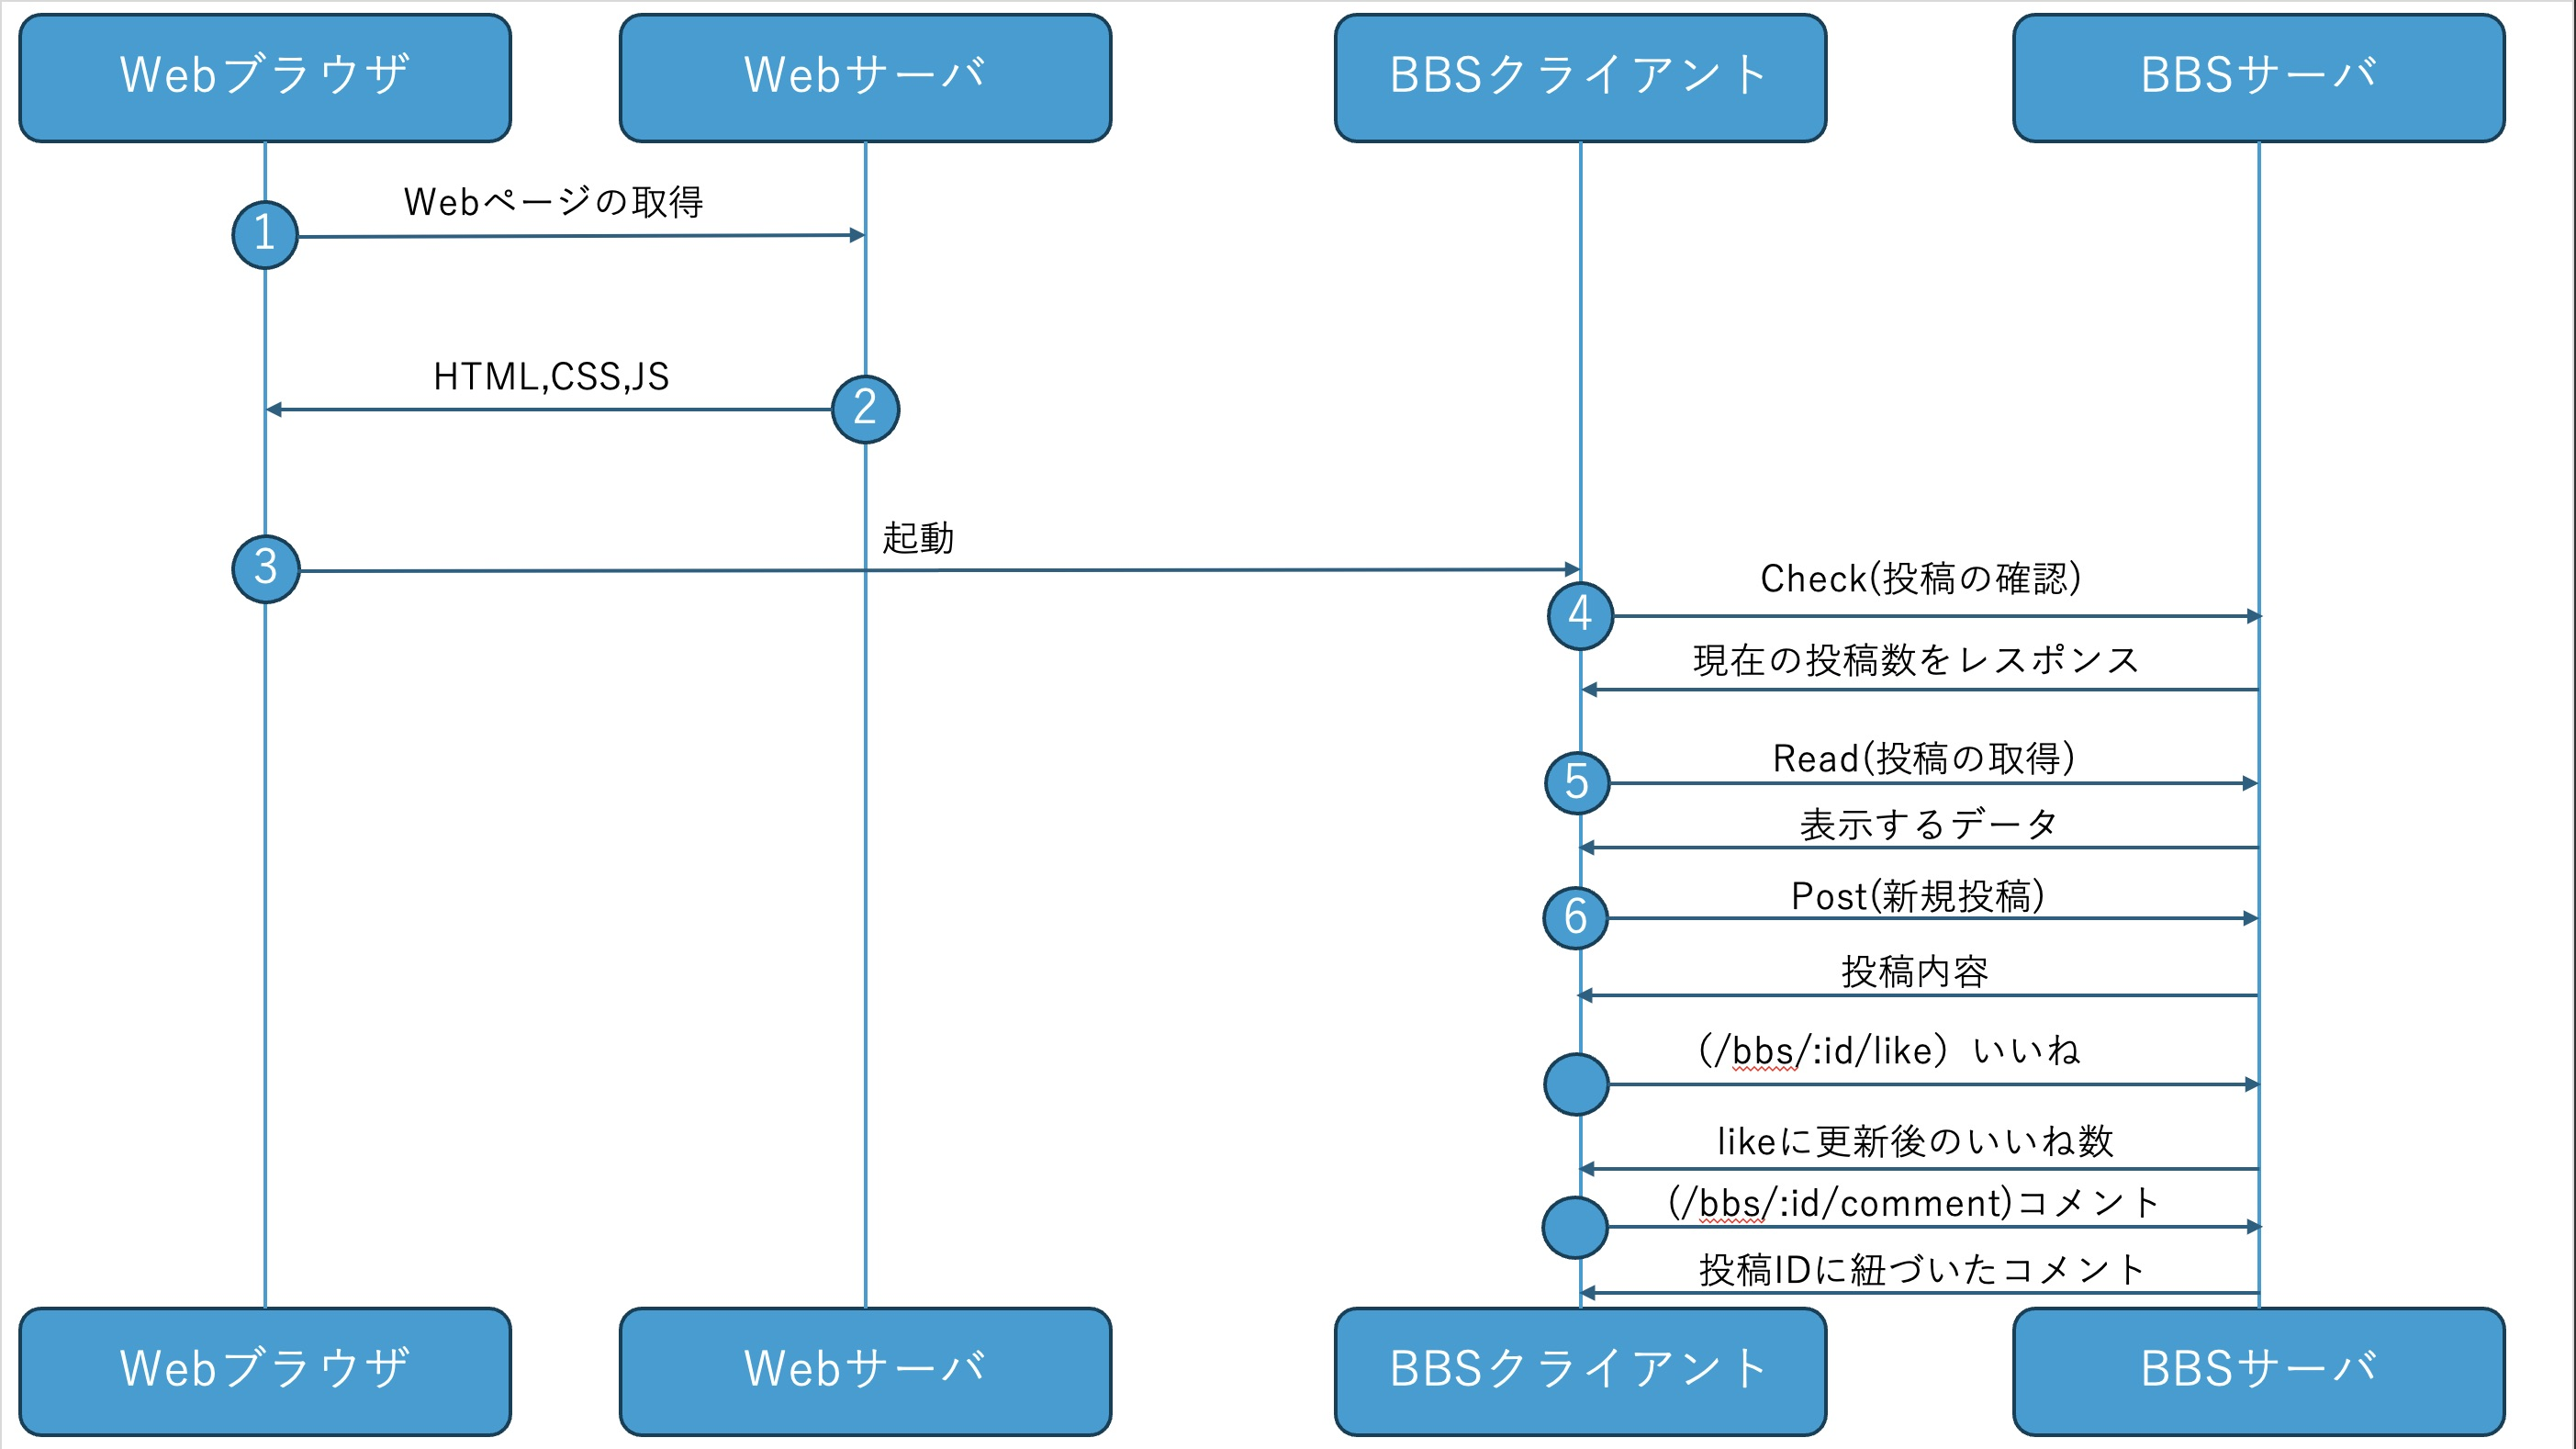
\includegraphics[width=10cm]{fig/zu.jpeg}
    \caption{機能}
    \label{photoreflector_characteristic}
\end{figure}

\par
github: https://github.com/Sou0202/webpro_06

\end{document}